
\de{ĐỀ THI GIỮA HỌC KỲ I NĂM HỌC 2023-2024}{THPT HÙNG VƯƠNG }
\begin{center}
	\textbf{PHẦN 1 - TRẮC NGHIỆM}
\end{center}
\Opensolutionfile{ans}[ans/ans]

\begin{ex}%[0D1Y3-1]%[Dự án đề kiểm tra Toán 10 GHKI NH23-24- Nguyễn Hoài Nam]%[THPT Hùng Vương]
Cho hai tập hợp $A=\left\{-2;-1;0;1;2;3;4;5\right\}$ và $A=\left\{-4;-3;-2;-1;0;1\right\}$. Tìm mệnh đề đúng.
\choice
{$A\cup B = \left\{-2;-1;0;1\right\}$}
{$A\cup B = \left\{-2;-1;0;1;2;3;4;5\right\}$}
{$A\cup B = \left\{-4;-3\right\}$}
{\True $A\cup B = \left\{-4;-3;-2;-1;0;1;2;3;4;5\right\}$}
\loigiai{
Ta có $A\cup B = \left\{-4;-3;-2;-1;0;1;2;3;4;5\right\}$.
}
\end{ex}

\begin{ex}%[0D1Y3-1]%[Dự án đề kiểm tra Toán 10 GHKI NH23-24- Nguyễn Hoài Nam]%[THPT Hùng Vương]
	Cho tập hợp $A=\left\{x \in \mathbb{N} \ | \ x\leq 5\right\}$. Tìm mệnh đề đúng.
	\choice
	{$A = \left\{1;2;3;4;5\right\}$}
	{$A = \left\{0;1;2;3;4\right\}$}
	{\True $A = \left\{0;1;2;3;4;5\right\}$}
	{$A = \left\{1;2;3;4\right\}$}
	\loigiai{
		Ta có $A=\left\{x \in \mathbb{N} \ | \ x\leq 5\right\} = \left\{0;1;2;3;4;5\right\}$.
	}
\end{ex}

\begin{ex}%[0H2Y1-3]%[Dự án đề kiểm tra Toán 10 GHKI NH23-24- Nguyễn Hoài Nam]%[THPT Hùng Vương]
	Gọi $O$ là giao điểm của hai đường chéo của hình bình hành $ABCD$. Đẳng thức nào sau đây \textbf{sai}?
	\choice
	{$\overrightarrow{AB}=\overrightarrow{DC}$}
	{$\overrightarrow{CB}=\overrightarrow{DA}$}
	{\True $\overrightarrow{OA}=\overrightarrow{OC}$}
	{$\overrightarrow{OB}=\overrightarrow{DO}$}
	\loigiai{
		\immini{
			Đẳng thức sai là $\overrightarrow{OA}=\overrightarrow{OC}$.}
		{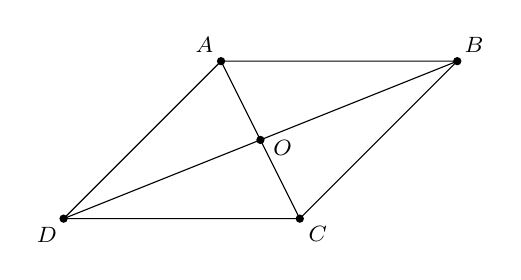
\begin{tikzpicture}[scale=1, font=\footnotesize, line join=round, line cap=round, >=stealth]
				\path 
				(2,2) coordinate (A)
				(5,2) coordinate (B)
				(3,0) coordinate (C)
				(0,0) coordinate (D)
				(2.5,1) coordinate (O)
				;
				
				\draw (A)--(B)--(C)--(D)--cycle (A)--(C) (B)--(D);
				
				\foreach \p/\r in {A/135,B/45,C/-40,D/-135,O/-20}
				\fill (\p) circle (1.5pt) node[shift={(\r:3mm)}]{$\p$};
		\end{tikzpicture}}
		
	}
\end{ex}

\begin{ex}%[0D1Y3-1]%[Dự án đề kiểm tra Toán 10 GHKI NH23-24- Nguyễn Hoài Nam]%[THPT Hùng Vương]
	Cho biểu đồ Venn sau đây, phần được tô màu biểu diễn tập hợp nào?
	\begin{center}
		\begin{tikzpicture}
			\def\firstcircle{(0:0) circle (1.2cm)}
			\def\secondcircle{(0:1.8) circle (1.2cm)}
			\begin{scope}
				\clip \secondcircle;
				\fill[pattern=north east lines, yellow] \firstcircle;
			\end{scope}
			\draw \firstcircle node[left]{$A$};
			\draw \secondcircle node [right]{$B$};
			%\node[below] () at (0.9,-1.5){$A\cap B$ là phần tô màu vàng};
		\end{tikzpicture}
	\end{center}
	\choice
	{$B\setminus A$}
	{$A \setminus B$}
	{\True $A \cap B$}
	{$A \cup B$}
	\loigiai{
		Phần được tô màu biểu diễn tập hợp $A \cap B$.
	}
\end{ex}

\begin{ex}%[0H2Y2-2]%[Dự án đề kiểm tra Toán 10 GHKI NH23-24- Nguyễn Hoài Nam]%[THPT Hùng Vương]
	Cho hình bình hành $ABCD$. Khẳng định nào sau đây đúng?
	\choice
	{$\overrightarrow{AB}+\overrightarrow{AC}=\overrightarrow{AD}$}
	{$\overrightarrow{AB}+\overrightarrow{AC}=\overrightarrow{CB}$}
	{$\overrightarrow{AB}-\overrightarrow{AC}=\overrightarrow{DA}$}
	{$\overrightarrow{AB}-\overrightarrow{AC}=\overrightarrow{BC}$}
	\loigiai{
		\immini{Khẳng định đúng là $\overrightarrow{AB}-\overrightarrow{AC}=\overrightarrow{DA}$.}
		{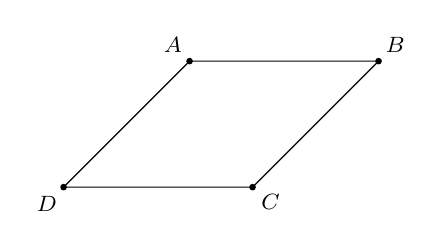
\begin{tikzpicture}[scale=0.8, font=\footnotesize, line join=round, line cap=round, >=stealth]
				\path 
				(2,2) coordinate (A)
				(5,2) coordinate (B)
				(3,0) coordinate (C)
				(0,0) coordinate (D)
				(2.5,1) coordinate (O)
				;
				
				\draw (A)--(B)--(C)--(D)--cycle ;
				
				\foreach \p/\r in {A/135,B/45,C/-40,D/-135}
				\fill (\p) circle (1.5pt) node[shift={(\r:3mm)}]{$\p$};
		\end{tikzpicture}}
		
	}
\end{ex}
\begin{ex}%[0H4B2-1]%[Dự án đề kiểm tra Toán 10 GHKI NH23-24- Nguyễn Hoài Nam]%[THPT Hùng Vương]
	Cho tam giác $ABC$ với $a=BC$, $b=AC$, $c=AB$, $S$ là diện tích tam giác $ABC$, $R$ là bán kính đường tròn ngoại tiếp tam giác $ABC$. Khẳng định nào sau đây là đúng?
	\choice
	{\True$\cos C=\dfrac{b^2+a^2-c^2}{2ab}$}
	{$S=\dfrac{1}{2}abc$}
	{$\cos B=\dfrac{b^2+c^2-a^2}{2bc}$}
	{$\dfrac{a}{\sin A}=R$}
	\loigiai{
		Ta có $\cos C=\dfrac{b^2+a^2-c^2}{2ab}$
	}
\end{ex}

\begin{ex}%[0D2N1-2]%[Dự án đề kiểm tra Toán 10 GHKI NH23-24- Nguyễn Hoài Nam]%[THPT Hùng Vương]
	Cặp số nào là một nghiệm của bất phương trình $-5x-y>6$?
	\choice
	{$(4;-2)$}
	{$(-1;1)$}
	{$(1;3)$}
	{\True $(-3;0)$}
	\loigiai{
		Ta có $-5 \cdot (-3)-0=15>6$ nên $(-3;0)$ là nghiệm của bất phương trình.
	}
\end{ex}		

\begin{ex}%[0H4B1-3]%[Dự án đề kiểm tra Toán 10 GHKI NH23-24- Nguyễn Hoài Nam]%[THPT Hùng Vương]
	Trong các đẳng thức sau đây, đẳng thức nào đúng?
	\choice
	{$\tan (180^\circ -\alpha)=\tan \alpha$}
	{\True $\cot (180^\circ -\alpha)=-\cot \alpha$}
	{$\sin (180^\circ -\alpha)=-\sin \alpha$}
	{$\cos (180^\circ -\alpha)=\cos \alpha$}
	\loigiai{
		Ta có $\cot (180^\circ -\alpha)=-\cot \alpha$.
	}
\end{ex}
\begin{ex}%[0D2B1-2]%[Dự án đề kiểm tra Toán 10 GHKI NH23-24- Nguyễn Hoài Nam]%[THPT Hùng Vương]
	Miền nghiệm của bất phương trình $x+y\le 2$ (phần không bị gạch) được biểu diễn bởi hình vẽ nào dưới đây?
	\choice
	{
		\begin{tikzpicture}[scale=.8,xscale=.7,yscale=.7,font=\footnotesize,line join=round,line cap=round,>=stealth]
			\draw[->] (-1,0) -- (3,0) node[right] {$x$};
			\draw[->] (0,-1) -- (0,3) node[above] {$y$};
			\fill[domain=-1:3,samples=100,pattern=north east lines] (-1,-1)--plot(\x,{2-\x})--(3,-1)--cycle;
			\draw[domain=-1:3,samples=100] plot(\x,{2-\x});
			\draw[fill=black] (0,0)node[below left]{$O$}circle(1pt) (2,0)node[above]{$2$}circle(1pt) (0,2)node[right]{$2$}circle(1pt);
		\end{tikzpicture}
	}
	{\True 
		\begin{tikzpicture}[scale=.8,xscale=.7,yscale=.7,font=\footnotesize,line join=round,line cap=round,>=stealth]
			\draw[->] (-1,0) -- (3,0) node[right] {$x$};
			\draw[->] (0,-1) -- (0,3) node[above] {$y$};
			\fill[domain=-1:3,samples=100,pattern=north east lines] (3,-1)--plot(\x,{2-\x})--(-1,3)--(3,3)--cycle;
			\draw[domain=-1:3,samples=100] plot(\x,{2-\x});
			\draw[fill=black] (0,0)node[below left]{$O$}circle(1pt) (2,0)node[below]{$2$}circle(1pt) (0,2)node[left]{$2$}circle(1pt);
		\end{tikzpicture}
	}
	{
		\begin{tikzpicture}[scale=.8,xscale=.7,yscale=.7,font=\footnotesize,line join=round,line cap=round,>=stealth]
			\draw[->] (-3,0) -- (1,0) node[below] {$x$};
			\draw[->] (0,-1) -- (0,3) node[left] {$y$};
			\fill[domain=-3:1,samples=100,pattern=north west lines] (-3,-1)--plot(\x,{2+\x})--(1,3)--(1,-1)--cycle;
			\draw[domain=-3:1,samples=100] plot(\x,{2+\x});
			\draw[fill=black] (0,0)node[below left]{$O$}circle(1pt) (-2,0)node[above]{$-2$}circle(1pt) (0,2)node[left]{$2$}circle(1pt);
		\end{tikzpicture}
	}
	{
		\begin{tikzpicture}[scale=.8,xscale=.7,yscale=.7,font=\footnotesize,line join=round,line cap=round,>=stealth]
			\draw[->] (-3,0) -- (1,0) node[right] {$x$};
			\draw[->] (0,-1) -- (0,3) node[above] {$y$};
			\fill[domain=-3:1,samples=100,pattern=north west lines] (-3,-1)--plot(\x,{2+\x})--(1,3)--(-3,3)--cycle;
			\draw[domain=-3:1,samples=100] plot(\x,{2+\x});
			\draw[fill=black] (0,0)node[below left]{$O$}circle(1pt) (-2,0)node[below]{$-2$}circle(1pt) (0,2)node[right]{$2$}circle(1pt);
		\end{tikzpicture}
	}
	\loigiai{
		Đường thẳng $x+y=2$ đi qua hai điểm $(2;0)$ và $(0;2)$. \\
		Thay $x=0$, $y=0$ vào bất phương trình ta được $0+0\le 2$ đúng. Do đó miền nghiệm của bất phương trình là miền chứa gốc tọa độ $O$.
	}
\end{ex}

\begin{ex}%[0D2B1-2]%[Dự án đề kiểm tra Toán 10 GHKI NH23-24- Nguyễn Hoài Nam]%[THPT Hùng Vương]
	Phủ định của mệnh đề $P \colon $\lq\lq $\exists x \in \mathbb{N} \colon x^2-3x+2=0$\rq\rq \ là
	\choice
	{$\overline{P} \colon$\lq\lq $\exists x \in \mathbb{N} \colon x^2-3x+2 \ne 0$\rq\rq}
	{$\overline{P} \colon$\lq\lq $\forall x \in \mathbb{N} \colon x^2-3x+2 = 0$\rq\rq}
	{$\overline{P} \colon$\lq\lq $\forall x \in \mathbb{N} \colon x^2-3x+2 > 0$\rq\rq}
	{\True $\overline{P} \colon$\lq\lq $\forall x \in \mathbb{N} \colon x^2-3x+2 \ne 0$\rq\rq}
	\loigiai{
		Ta có $\overline{P} \colon$\lq\lq $\forall x \in \mathbb{N} \colon x^2-3x+2 \ne 0$\rq\rq.
	}
\end{ex}

\Closesolutionfile{ans}
%\begin{center}
%	\textbf{ĐÁP ÁN}
%	\inputansbox{10}{ans/ans}	
%\end{center}
\begin{center}
	\textbf{PHẦN 2 - TỰ LUẬN}
\end{center}

\begin{bt}%[0D2B1-2]%[Dự án đề kiểm tra Toán 10 GHKI NH23-24- Nguyễn Hoài Nam]%[THPT Hùng Vương]
	Cho $A=(-1;5)$, $B=[2;+\infty)$. Xác định các tập hợp $A \cup B$, $A \setminus B$ và biểu diễn trên trục số.
	\loigiai{
		$A\cup B=(-1;+\infty)$. Biểu diễn trên trục số
		\begin{center}
			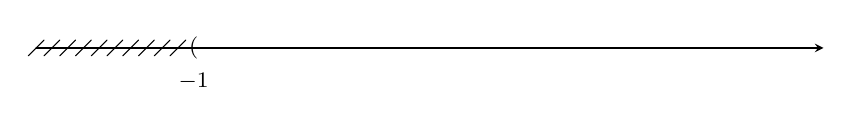
\begin{tikzpicture}[scale=1, font=\footnotesize, line join=round, line cap=round, >=stealth]
				\draw[->] (-3,0)--(7,0);
				\path (-1,0) node{$($} (-1,-0.2) node[below]{$-1$};
				\foreach \x in {-3,-2.8,...,-1.2}\draw(\x-0.1,-0.1)--(\x+0.1,0.1);
			\end{tikzpicture}
		\end{center}
	$A \setminus B =(-1;2)$. Biểu diễn trên trục số
		\begin{center}
			
\begin{tikzpicture}[scale=1, font=\footnotesize, line join=round, line cap=round, >=stealth]
				\draw[->] (-3,0)--(7,0);
				\path (-1,0) node{$($} (-1,-0.2) node[below]{$-1$}
				(2,0) node{$)$} (2,-0.2) node[below]{$2$};
				\foreach \x in {-3,-2.8,...,-1.2, 2.2,2.4,...,6.8}\draw(\x-0.1,-0.1)--(\x+0.1,0.1);
			\end{tikzpicture}
		\end{center}
	}
\end{bt}
\begin{bt}%[0H4B3-1]%[Dự án đề kiểm tra Toán 10 GHKI NH23-24- Nguyễn Hoài Nam]%[THPT Hùng Vương]
	Cho tam giác $ABC$ có $BC=3$, $AC=5$ và $\widehat{ACB}=60^{\circ}$.
	\begin{enumerate}
		\item Tính độ dài cạnh $AB$ của tam giác $ABC$.
		\item Tính diện tích tam giác $ABC$.
	\end{enumerate}
	\loigiai{
		\immini{\begin{enumerate}
				\item Áp dụng định lý cô-sin ta có
				\begin{eqnarray*}
					&&AB^2=CB^2+CA^2-2\cdot CB \cdot CA \cdot \cos \widehat{ACB}=31 \\
					&&\Rightarrow AB=\sqrt{31}.
				\end{eqnarray*}
				\item Ta có $S_{\triangle ABC}= \dfrac{1}{2}CA \cdot CB \cdot \sin \widehat{ACB}=\dfrac{15}{4}$.
		\end{enumerate}}
		{\begin{tikzpicture}[scale=1, font=\footnotesize, line join=round, line cap=round, >=stealth]
				\path 
				(0,0) coordinate (A)
				(3.83,2.03) coordinate (B)
				(5,0) coordinate (C)
				;
				
				\draw (A)--(B)--(C)--cycle;
				
				\foreach \p/\r in {A/180,B/45,C/0}
				\fill (\p) circle (1.5pt) node[shift={(\r:3mm)}]{$\p$};
				\draw    pic["$60^\circ$", draw=black, -, angle eccentricity=1.5, angle radius=0.5cm]
				{ angle=B--C--A};
		\end{tikzpicture}}
		
	}
\end{bt}

\begin{bt}%[[0H5B1-5]%[Dự án đề kiểm tra Toán 10 GHKI NH23-24- Nguyễn Hoài Nam]%[THPT Hùng Vương]
	Cho tam giác đều $ABC$ cạnh $a$.
	\begin{enumerate}
		\item Tính độ dài véc-tơ $\overrightarrow{AB}+\overrightarrow{AC}$.
		\item Gọi $M$ là một điểm trên cạnh $BC$ sao cho $MB=2MC$. Chứng minh rằng $\overrightarrow{AM}=\dfrac{1}{3}\overrightarrow{AB}+\dfrac{2}{3}\overrightarrow{AC}$.
	\end{enumerate}
	\loigiai{
		\begin{center}
			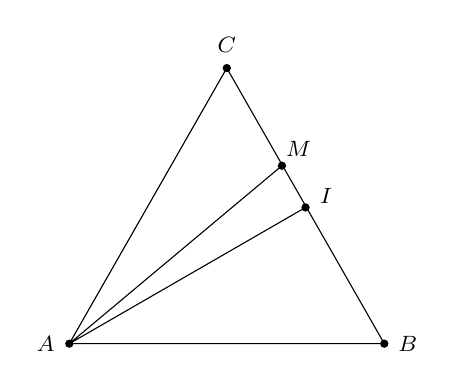
\begin{tikzpicture}[scale=1, font=\footnotesize, line join=round, line cap=round, >=stealth]
			\path 
			(-6,3) coordinate (A)
			(-2,3) coordinate (B)
			(-4,6.5) coordinate (C)
			(-3.3,5.26) coordinate (M)
			(-3,4.73) coordinate (I)
			;
			
			\draw (A)--(B)--(C)--cycle (A)--(M) (A)--(I);
			
			\foreach \p/\r in {A/180,B/0,C/90,M/45,I/30}
			\fill (\p) circle (1.5pt) node[shift={(\r:3mm)}]{$\p$};
		\end{tikzpicture}
		\end{center}
		\begin{enumerate}
			\item Ta có $\overrightarrow{AB}+\overrightarrow{AC}=2\overrightarrow{AI}$ với $I$ là trung điểm của đoạn thẳng $BC$. \\
			Từ đó ta có $\left|\overrightarrow{AB}+\overrightarrow{AC} \right| =2AI$.\\
			Mà $AI$ là đường trung tuyến (cũng là đường cao) trong tam giác đều cạnh $a$ nên $AI=\dfrac{a\sqrt{3}}{2}$. Do đó$\left|\overrightarrow{AB}+\overrightarrow{AC} \right| =2AI=\sqrt{3}$.
			\item $M$ nằm trên cạnh $BC$ nên ta có 
			\begin{eqnarray*}
				\overrightarrow{MB}=-2\overrightarrow{MC} &\Leftrightarrow& \overrightarrow{AB}-\overrightarrow{AM} = -2(\overrightarrow{AC}-\overrightarrow{AM})\\ &\Leftrightarrow& 3\overrightarrow{AM}=\overrightarrow{AB}+2\overrightarrow{AC} \\
				&\Leftrightarrow& \overrightarrow{AM}=\dfrac{1}{3}\overrightarrow{AB} + \dfrac{2}{3}\overrightarrow{AC}.
			\end{eqnarray*}
		\end{enumerate}
	}
\end{bt}

\begin{bt}%[0H4K3-2]%[Dự án đề kiểm tra Toán 10 GHKI NH23-24- Nguyễn Hoài Nam]%[THPT Hùng Vương]
	\immini{Một cây cổ thụ mọc thẳng đứng bên lề một con dốc có độ dốc $8^{\circ}$ so với phương nằm ngang. Từ một điểm dưới chân dốc, cách gốc cây $28$ m người ta nhìn thấy đỉnh ngọn cây dưới một góc $40^{\circ}$ so với phương ngang. Tính chiều cao của cây đó.
		(Làm tròn đến hàng đơn vị, theo đơn vị mét).}
	{
		\usetikzlibrary{decorations.pathmorphing,shapes}
		\tikzset{
			treetop/.style = {
				decoration={random steps, segment length=0.4mm},
				decorate
			},
			trunk/.style = {
				decoration={random steps, segment length=2mm, amplitude=0.2mm},
				decorate
			}
		}
		\tikzset{
			man/.pic={%
				\fill [rounded corners=1.5] (0,0.4) -- (0,0.4 -- (0.4,0.5 -- (0.4,0.4) --
				(0.325,0.4) -- (0.325,0.7) -- (0.3,0.7) -- (0.3,0) -- (0.225,0) --
				(0.225,0.4) -- (0.175,0.4) -- (0.175,0) -- (0.1,0) -- (0.1,0.7) --
				(0.075,0.7) -- (0.075,0.4) -- cycle;
				\fill (0.2,0.9) circle (0.1);
				\coordinate (-head) at (0.2,1);
				\coordinate (-foot) at (0.2,0);
			}
		}
		\begin{tikzpicture}
			\path 
			(0,1.5) coordinate (C)
			(-5,-5) coordinate (H)
			(0,-3) coordinate (B)
			(0,-5) coordinate (B1)		
			;
			%\pic[red] at (-6.3,-3) (myman) {man};
			\foreach \w/\f in {0.3/30,0.2/50,0.1/70} {
				\fill [brown!\f!black, trunk] (0,0) ++(-\w/2,0) rectangle +(\w,-3);
			}
			\foreach \n/\f in {1.4/40,1.2/50,1/60,0.8/70,0.6/80,0.4/90} {
				\fill [green!\f!black, treetop] ellipse (\n/1.5 and \n);
			}
			\draw (B)--(B1)--(H)--(C)  (B)--(H);
			\pic[draw,"$8^{\circ}$", angle eccentricity=1.4,angle radius=0.8cm]{angle=B1--H--B};
			\pic[draw,"$40^{\circ} $", angle eccentricity=1.4,angle radius=0.7cm]{angle=B1--H--C};
			\draw pic[draw, angle radius=2mm]{right angle=B--B1--H};
			\path (H)--(B) node[below,midway,sloped]{$28$ m};
			%	\foreach \x/\g in {} \fill[black] (\x)+(\g:.3) node {$\x$};
		\end{tikzpicture}
	}
	\loigiai{
		\immini{
			Đặt tên các điểm $B$, $H$, $C$, $A$ như hình vẽ.\\
			Khi đó $BC$ là chiều cao của cây.\\
			Theo đề ta có $\widehat{BHA}=8^{\circ}$, $\widehat{CHA}=40^{\circ}$, từ đó ta có $\widehat{CHB}=32^{\circ}$. \\
			Bên cạnh đó ta có tam giác $BHA$ vuông tại $A$ nên $\widehat{ABH}=82^{\circ}$.\\
			Mà $\widehat{CBH}+\widehat{ABH}=180^{\circ}$ nên $\widehat{CBH}=98^{\circ}$.\\
			Ta có $\widehat{CHB}+ \widehat{CBH}+\widehat{BHC}=180^{\circ} \Rightarrow \widehat{BHC}=50^{\circ}$.
			Áp dụng định lý $\sin$ vào tam giác $BCH$ ta có
			\begin{eqnarray*}
				&&\dfrac{BC}{\sin \widehat{CHB}}=\dfrac{HB}{\sin \widehat{BCH}} \\
				&\Rightarrow& BC=\dfrac{HB \sin \widehat{CHB}}{\sin \widehat{BCH}}=\dfrac{28 \cdot \sin 32^{\circ}}{\sin 50^{\circ}}\approx 19 \ (\mathrm{m}).
			\end{eqnarray*}
			
		}{
			\usetikzlibrary{decorations.pathmorphing,shapes}
			\tikzset{
				treetop/.style = {
					decoration={random steps, segment length=0.4mm},
					decorate
				},
				trunk/.style = {
					decoration={random steps, segment length=2mm, amplitude=0.2mm},
					decorate
				}
			}
			\tikzset{
				man/.pic={%
					\fill [rounded corners=1.5] (0,0.4) -- (0,0.4 -- (0.4,0.5 -- (0.4,0.4) --
					(0.325,0.4) -- (0.325,0.7) -- (0.3,0.7) -- (0.3,0) -- (0.225,0) --
					(0.225,0.4) -- (0.175,0.4) -- (0.175,0) -- (0.1,0) -- (0.1,0.7) --
					(0.075,0.7) -- (0.075,0.4) -- cycle;
					\fill (0.2,0.9) circle (0.1);
					\coordinate (-head) at (0.2,1);
					\coordinate (-foot) at (0.2,0);
				}
			}
			\begin{tikzpicture}
				\path 
				(0,1.5) coordinate (C)
				(-5,-5) coordinate (H)
				(0,-3) coordinate (B)
				(0,-5) coordinate (A)		
				;
				%\pic[red] at (-6.3,-3) (myman) {man};
				\foreach \w/\f in {0.3/30,0.2/50,0.1/70} {
					\fill [brown!\f!black, trunk] (0,0) ++(-\w/2,0) rectangle +(\w,-3);
				}
				\foreach \n/\f in {1.4/40,1.2/50,1/60,0.8/70,0.6/80,0.4/90} {
					\fill [green!\f!black, treetop] ellipse (\n/1.5 and \n);
				}
				\draw (B)--(A)--(H)--(C)  (B)--(H);
				\pic[draw,"$8^{\circ}$", angle eccentricity=1.4,angle radius=0.8cm]{angle=A--H--B};
				\pic[draw,"$40^{\circ} $", angle eccentricity=1.4,angle radius=0.7cm]{angle=A--H--C};
				\draw pic[draw, angle radius=2mm]{right angle=B--A--H};
				\path (H)--(B) node[below,midway,sloped]{$28$ m};
				\foreach \t/\g in {A/-90,C/90,B/0,H/180}{\draw[fill=white] (\t) circle (1pt) node[shift={(\g:8pt)},font=\footnotesize]{$ \t $};}
			\end{tikzpicture}
		}
	}
\end{bt}
